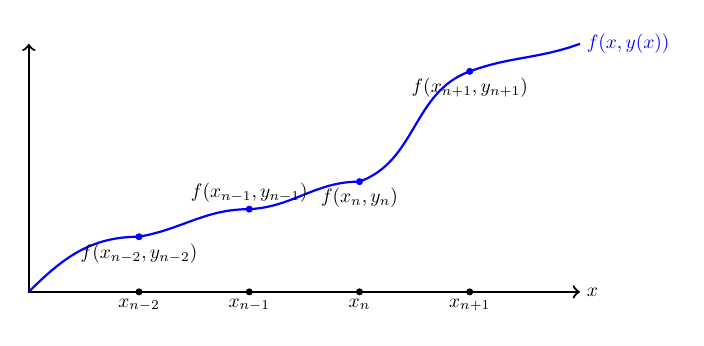
\begin{tikzpicture}[scale=0.7,every node/.style={scale=0.7}]
	% Ejes
	\draw [thick, <->] (0,4.5) -- (0,0) -- (10,0);
	% f(x_n,y_n)
	\draw[blue,thick] (0,0) to[out=45,in=180] (2,1);
	\draw[blue,thick] (2,1) to[out=10,in=180] (4,1.5);
	\draw[blue,thick] (4,1.5) to[out=3,in=180] (6,2);
	\draw[blue,thick] (6,2) to[out=20,in=200] (8,4);
	\draw[blue,thick] (8,4) to[out=20,in=200] (10,4.5);
	% Labels x_n
	\draw[fill] (2,0) circle [radius=1.5pt];
	\node[below] at (2,0) {$x_{n-2}$};
	\draw[fill] (4,0) circle [radius=1.5pt];
	\node[below] at (4,0) {$x_{n-1}$};
	\draw[fill] (6,0) circle [radius=1.5pt];
	\node[below] at (6,0) {$x_{n}$};
	\draw[fill] (8,0) circle [radius=1.5pt];
	\node[below] at (8,0) {$x_{n+1}$};
	% Lables fs
	\draw[blue, fill] (2,1) circle [blue,radius=1.5pt];
	\node[font=\fontsize{10}{144}\selectfont, below] at (2,1) {$f(x_{n-2},y_{n-2})$};
	\draw[blue, fill] (4,1.5) circle [blue,radius=1.5pt];
	\node[font=\fontsize{10}{144}\selectfont, above] at (4,1.5) {$f(x_{n-1},y_{n-1})$};
	\draw[blue, fill] (6,2) circle [blue,radius=1.5pt];
	\node[font=\fontsize{10}{144}\selectfont, below] at (6,2) {$f(x_{n},y_{n})$};
	\draw[blue, fill] (8,4) circle [blue,radius=1.5pt];
	\node[font=\fontsize{10}{144}\selectfont, below] at (8,4) {$f(x_{n+1},y_{n+1})$};
	% General labels
	\node[right] at (10,0) {$x$};
	\node[blue,right] at (10,4.5) {$f(x,y(x))$};
\end{tikzpicture}